\renewcommand*{\authorOfNextLines}{Helmut Quinz}
Der Speicherort der zu dieser Vorlage gehörenden Dateien ist unerheblich.
Es empfiehlt sich aber ein Verzeichnis auf einem Cloud-Speicher zu verwenden.
Das reduziert die Gefahr Daten zu verlieren und ermöglicht dezentrales Arbeiten.
Innerhalb des Verzeichnisses wird empfohlen folgende Struktur beizubehalten:
\begin{figure} [ht]
	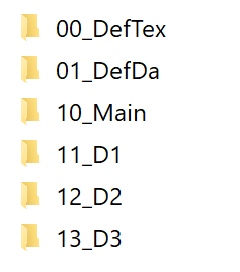
\includegraphics{../13_D3/VorlageDateistruktur.png} 
	\caption{Verzeichnisstruktur dieser Vorlage}
\end{figure}
\FloatBarrier
Die Verzeichnisse sind wie folgt festgelegt:
\begin {table} [ht]
\stretchTableRows{1.3}
\begin{tabular}{p{20mm}p{37mm}p{90mm}}
	Verzeichnis 		& Inhalt  	& Bemerkung\\ \hline
	\texttt{00\_DefTex}	& Für den Aufbau des Dokuments relevante Definitionen 
		& Der Verzeichnisname wird von der Vorlage referenziert und darf nicht verändert werden.
		  Der Inhalt des Ordners ist nur in Ausnahmefällen zu ändern.\\
	\texttt{01\_DefDa}	& Einstellungen zur \typeOfWork ~.  
		& Der Verzeichnisname wird von der Vorlage referenziert und darf nicht verändert werden.
		  Der Inhalt der Dateien in diesem Ordner ist vom Anwender der Arbeit entsprechend anzupassen.\\
	\texttt{10\_Main}	& Hauptdokument	
		& Änderungen im Verzeichnis- und Dokumentnamen haben bei korrektem Arbeiten keine Auswirkung.
		  Das Hauptdokument muss jedoch direkt in einem Unterverzeichnis abgelegt sein.\\
	\texttt{11\_D1}	& von den Anwendern erstellte Dateien, Inhalt der \typeOfWork .	
		& Änderungen im Verzeichnis- und Dokumentnamen haben bei korrektem Arbeiten keine Auswirkung.
		  Die Strukturierung ist nur ein Vorschlag des Autors. 
		  Die einzelnen Dokumente können auch unter \texttt{10\_Main} abgelegt sein.\\
\end{tabular}
\caption {Inhalt der Verzeichnisse dieser Vorlage}
\end {table}
\FloatBarrier
Grundsätzlich ist das Schreiben der kompletten \typeOfWork ~im Hauptdokument möglich.
Es erscheint jedoch praktikabel mehrere kleine Dateien zum Einbinden in das Hauptdokument anzulegen. 
Dies gestaltet Anpassungen der in Dokumentstruktur während dem Erstellen der Dokumentation einfacher!

\subsubsection{Hinweis:}
Anders als bei Windows-Systemen ist unter Linux die korrekte Groß- und Kleinschreibung bei Verzeichnis- und Dateinamen für das Finden der Dateien durch den Compiler relevant!